\documentclass[tikz,border=7pt]{standalone}
\usepackage{amsmath,pgfplots}
\pgfplotsset{compat=1.18}
\usetikzlibrary{arrows.meta}
\definecolor{ink}{HTML}{21352F}\definecolor{teal}{HTML}{087F7B}
\definecolor{gold}{HTML}{C58B2A}\definecolor{blue}{HTML}{4B77A8}\definecolor{rose}{HTML}{B65A62}
\begin{document}
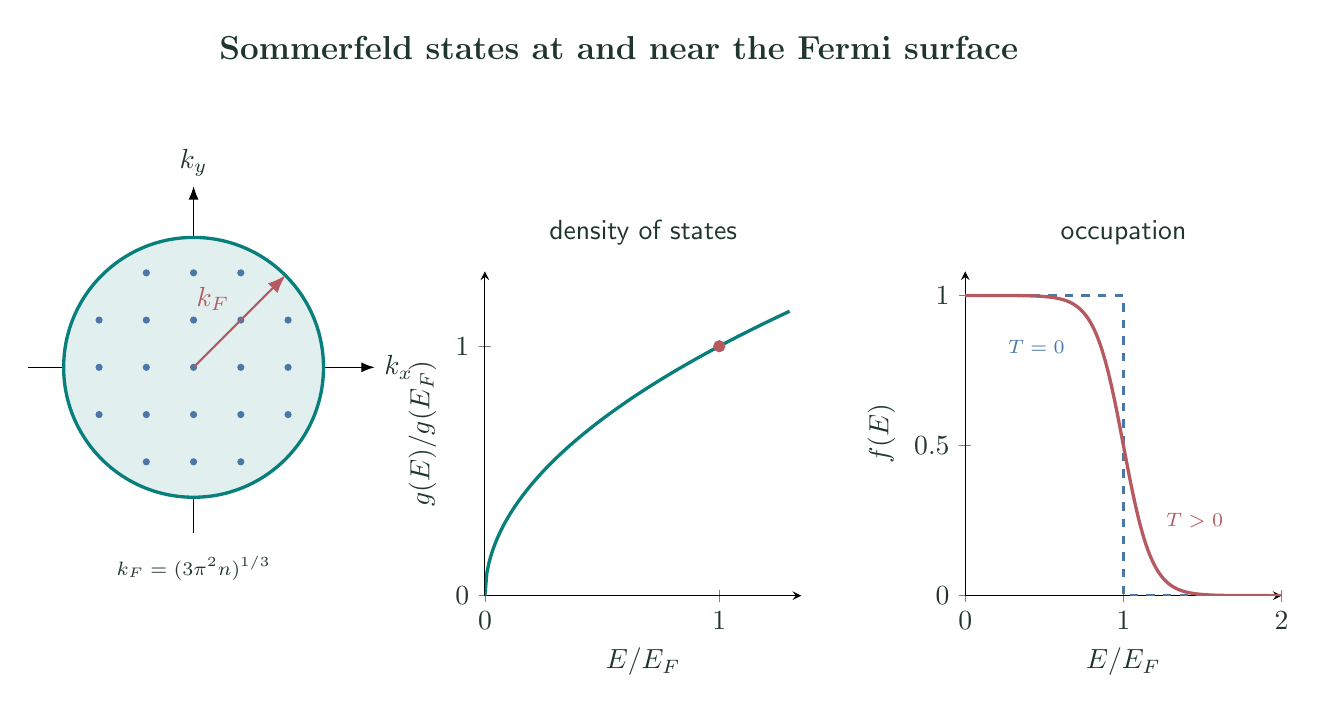
\begin{tikzpicture}[font=\sffamily,text=ink,>=Latex]
\node[font=\bfseries\large] at (0,4.3) {Sommerfeld states at and near the Fermi surface};
\begin{scope}[xshift=-5.4cm,yshift=.25cm]
 \draw[->] (-2.1,0)--(2.3,0) node[right] {$k_x$}; \draw[->] (0,-2.1)--(0,2.3) node[above] {$k_y$};
 \fill[teal!12] (0,0) circle (1.65); \draw[teal,very thick] (0,0) circle (1.65);
 \foreach \x in {-1.2,-.6,0,.6,1.2}\foreach \y in {-1.2,-.6,0,.6,1.2}{\pgfmathparse{\x*\x+\y*\y<2.45?1:0}\ifnum\pgfmathresult=1\fill[blue] (\x,\y) circle (1.3pt);\fi}
 \draw[->,rose,thick] (0,0)--(1.17,1.17) node[midway,above left] {$k_F$};
 \node[font=\scriptsize] at (0,-2.55) {$k_F=(3\pi^2n)^{1/3}$};
\end{scope}
\begin{axis}[at={(-1.7cm,-2.65cm)},anchor=south west,width=5.6cm,height=5.7cm,xmin=0,xmax=1.35,ymin=0,ymax=1.3,
 axis lines=left,xlabel={$E/E_F$},ylabel={$g(E)/g(E_F)$},xtick={0,1},ytick={0,1},title={density of states}]
 \addplot[teal,very thick,domain=0:1.3,samples=160]{sqrt(x)};
 \addplot[only marks,mark=*,rose] coordinates {(1,1)};
\end{axis}
\begin{axis}[at={(4.4cm,-2.65cm)},anchor=south west,width=5.6cm,height=5.7cm,xmin=0,xmax=2,ymin=0,ymax=1.08,
 axis lines=left,xlabel={$E/E_F$},ylabel={$f(E)$},xtick={0,1,2},ytick={0,.5,1},title={occupation}]
 \addplot[blue,dashed,very thick] coordinates {(0,1)(1,1)(1,0)(2,0)};
 \addplot[rose,very thick,domain=0:2,samples=200]{1/(exp((x-1)/.09)+1)};
 \node[font=\scriptsize,blue] at (axis cs:.45,.83) {$T=0$};
 \node[font=\scriptsize,rose] at (axis cs:1.45,.25) {$T>0$};
\end{axis}
\end{tikzpicture}
\end{document}

